\section{Simulated (stochastic) annealing}

\mode<presentation>{
\begin{frame} 
    \begin{center} \huge
        \secname
    \end{center}
	%\begin{center}
	%Dealing with the diverging hebbian rule\\
	%through implicit normalization
	
	%\end{center}
    \begin{center}
		\includegraphics[width=3cm]{img/380px-Blacksmith_anvil_hammer}
    \end{center}
\end{frame}
}

\begin{frame}{\secname}

\emph{Simulated annealing}\notesonly{\footnote{
The ``annealing'' part in the name comes from metallurgy. As metals cool down, the movement of the atoms slows down and their kinetic energy decreases until the metal eventually hardens.
}}
\notesonly{is a method for stochastic optimization with which we can find a tradeoff between exploitation and exploration. More importantly, it is designed to cope with optimization of discrete-valued arguments. Simulated annealing is
  motivated by phenomena in physics related to the organization and
  alignment of microscopic components forming specific macroscopic
  configurations. }
\slidesonly{\\$\leadsto$ exploitation and exploration tradeoff}
\slidesonly{\\$\leadsto$ (more importantly) discrete optimization\\\vspace{0.5cm}}

\end{frame}

\begin{frame}{\secname}

\svspace{-5mm}

\question{What does simulated annealing do?}

- In the case of \emph{minimization} it:

\begin{enumerate}
\item describes a strategy for switching between states
\item increases the probability of landing in lower-energy states\footnote{This preference for lower-energy states is specific to \emph{minimization} problems.}
\item allows for escaping \textbf{local} optima
\end{enumerate}


\begin{center}
	\includegraphics[width=5cm]{img/cyberscooty-switch_1-5_next}
\end{center}


\end{frame}

\begin{frame}
\slidesonly{
\frametitle{Simulated Annealing; the algorithm}

Use \emph{inverse} temperature $\beta = 1/T$\\\vspace{0.5cm}
}
\notesonly{
\textbf{Simulated Annealing, the algorithm}

We will use the inverse temperature $\beta = 1/T$\\\vspace{1cm}
}


\texttt{initialization:} $\vec{s}_0, \, \beta_0$ small ($\leadsto$ high temperature) \\

\texttt{BEGIN Annealing loop} ($t=1,2,\dots$)\\

\oident$\vec{s}_t = \vec{s}_{t-1}$ {\tiny(initialization of inner loop)} \\

\oident \texttt{BEGIN State update loop} ($M$ iterations)\\

\begin{itemize}
\item \texttt{choose a new candidate state} $\vec{s}$ randomly {(but ``close'' to $\vec{s}_t$)}\\

\item \texttt{calculate difference in cost:}
       \oident$\Delta E = E_{(\vec{s})}- E_{(\vec{s}_t)}$\\
\item 
\texttt{switch} $\vec{s}_t$ \texttt{to} $\vec{s}$ \texttt{ with probability} 
       $\color{red}\mathrm{W}_{(\vec{s}_t \rightarrow \vec{s})} =
	\frac{1}{1 + \exp( \beta_t \Delta E)}$
\texttt{\underline{otherwise} keep the previous state} $\vec{s}_t$
\end{itemize}
\oident\texttt{END State update loop} \\

\oident$\color{blue}\beta_t = \tau \beta_{t-1}\qquad $ {\footnotesize($\tau>1\implies$ increase of $\beta$)} \\ %  by practical ``exponential'' rule -- but not optimal

\texttt{END Annealing loop}

\end{frame}



\begin{frame} \frametitle{Transition probability}
% \vspace{-0.5cm} 
  \begin{center}\includegraphics[width=8cm]{img/section3_fig1}
  \end{center}
  \begin{center}
  \vspace{-0.5cm}
  $\mathrm{W}_{(\vec{s}_t \rightarrow \vec{s})} = \frac{1}{1 + \exp( \beta_t \Delta E)}, \quad \Delta E = E_{(\vec{s})}- E_{(\vec{s}_t)}$\\
  \end{center}
\end{frame}

\notesonly{
the transition probability $\mathrm{W}$ measures the probability of changing to a new state $\vec s$ or remaining at $\vec s_t$. It depends on (A) the difference in cost and (B) the inverse temperature. The difference $\Delta E$ is the only way of measuring whether we gain any improvement from the transition or not. We use the inverse temperature $\beta_t$ to control how much we favor such transitions, or if we prefer a more conservative system. Below illustrates how the transition probability can be modulated by the inverse temperature $\beta$ during the annealing process:
}

\begin{frame} \frametitle{Modulating $\mathrm W$ during the annealing process}
%  \textbf{ limiting cases for high vs.\ low temperature:}
  \begin{center}
    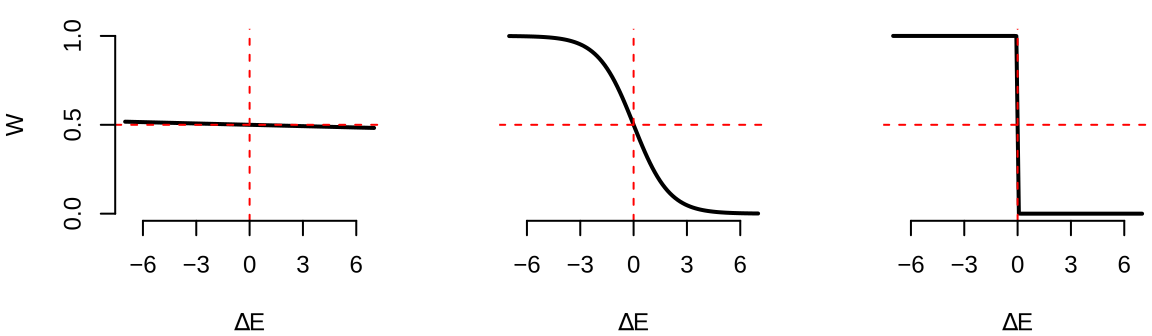
\includegraphics[width=10cm]{img/switchfuns}
\vspace{5mm}
  \oident\oident\begin{tabular}[h]{c c c}
    low $\beta$ (high temperature) & intermediate $\beta$  & high $\beta$\\\\
    \includegraphics[width=3cm]{img/section3_fig4}
    & \hspace{-0.5cm}\includegraphics[width=3cm]{img/section3_fig5}
    & \includegraphics[width=3cm]{img/section3_fig6}
  \end{tabular}
\vspace{5mm}
  \end{center}
  \vspace{-2cm}
  \begin{tikzpicture}[scale=0.75]
\draw[->] (0,0) -- (1,0);
\draw[->] (0,0) -- (0,1.25);
% \draw[lightgray, very thick] (-1,0.5) -- (.9,0.5);
% \draw (0,0) node[anchor=north]{0};
\draw (0,1.25) node[anchor=west]{$E$};
\draw (1,0) node[anchor=west]{$\vec{s}$};
% \foreach \y in {0.5,1} \draw (0,\y) node[anchor=south east] {$\y$};
% \foreach \y in {0.5,1} \draw (-1pt,\y) -- (1pt,\y);
\end{tikzpicture}

\question{Which range of $\beta$ corresponds to \emph{exploration}/\emph{exploitation}?}\\

\end{frame}

\notesonly{
In the case of:

\begin{itemize}
\item low $\beta \corresponds$ high temperature:\\
The transition probability is nearly constant (W=0.5) regardless of $\Delta E$. It is equally probably to accept a transition or to remain at the same state. Therefore we can regard this as \emph{exploration} mode.
\item intermediate $\beta$:\\
Recall that we are currently considering a minimization problem. $\Delta E < 0$ whenever the new state is of lower cost than the previous one. We are no longer indifferent to this difference, but are more likely to accept transitions to lower-energy-states. Our process is still stochastic, therefore it is not guaranteed that we will accept every transition that yileds lower lower cost. We may either reject the transition and remain at the same higher-cost state or accept a transition to higher-cost state. such transitions are less likely to happen, but are still possible. This is where stochastic optimization is able to escape a local optimum and resume the search elsewhere instead of opting for the greedy approach. To reiterate, this is a stochastic process, if we sample long enough, we will find that intermediate values of $\beta$ are more likely to yield samples from the ``global'' minimum of this curve than the higher ``local'' minimum in this particular cost function.
\item high $\beta \corresponds$ low temperature:\\
This is the \emph{exploitation} mode. This reflects the behavior of a greedy learning algorithm such as gradient descent. Whenever we compare the cost of two successive states and find that $\Delta E < 0$ it tells us that the new state is of lower cost and more desirable for our minimization objective. The transition probability in this case will almost always accept a transition to a lower-cost state. Consequently it will almost always reject transitions to high-cost states, and the probability of remaining in a high-cost state is also very low. If the next sample is of lower-cost, we are very likely to accept that transition. Looking again at the stochastic nature of our process: We repeat the process multiple times and register how often each \emph{run} (not a single iteration) leads us to either minimum on this particular curve, we will find that the chances of finding the global minimum is just as likely as those of reaching the local minimum. This is because the initial state is the only decisive factor. high $\beta$ means we are in exploitation mode. We are only going to accept a transition if it lowers our cost. If we restrict our sampling to ``nearby'' states, we are emulating gradient descent. As soon as we've determined the direction of descent, we will follow it. The decisive factor is, where did we start? Since in our case, the two valleys around the two minima are equally ``wide'', it makes starting inside one equal to starting inside the other. If I am already in the vicinity of one minimum, the probability of transitioning \emph{outside} is very low. This probability is low, regardless of whether I am in the vicinity of the global or local minimum.
\end{itemize}
}

\begin{frame}\frametitle{Annealing schedule \& convergence}
Convergence to the global optimum is guaranteed if $\beta_t \sim \ln (t)$\footnote{shown in \citep{geman1984stochastic}}

\begin{itemize}
	% \itR robust optimization procedure
	\itR but: $\beta_t \sim \ln t$ is \textbf{too slow} for practical problems
	\itR therefore: $\beta_{t+1} = \tau \beta_t, \quad \tau \in [1.01,1.30]$
		(exponential annealing)
	\itR additionally: the \texttt{State Update loop} has to be iterated often enough, e.g. $M=500-2000$. \slidesonly{$\leadsto$ thermal equilibrium}
	\notesonly{This is required for reaching thermal equilibrium. Another way to look at it is the need to capture the stationary distribution of the states in relation to their cost. We will talk more about when we discuss the Gibbs distribution.}
\end{itemize}
\end{frame}

\section{The stationary distribution}

\begin{frame}


\slidesonly{
  \begin{center}
  \oident\oident\begin{tabular}[h]{c c c}
    low $\beta$ (high temperature) & intermediate $\beta$  & high $\beta$\\\\
    \includegraphics[width=3cm]{img/section3_fig4}
    & \hspace{-0.5cm}\includegraphics[width=3cm]{img/section3_fig5}
    & \includegraphics[width=3cm]{img/section3_fig6}
  \end{tabular}
\vspace{5mm}
  \end{center}
  \vspace{-2cm}
  \begin{tikzpicture}[scale=0.75]
\draw[->] (0,0) -- (1,0);
\draw[->] (0,0) -- (0,1.25);
% \draw[lightgray, very thick] (-1,0.5) -- (.9,0.5);
% \draw (0,0) node[anchor=north]{0};
\draw (0,1.25) node[anchor=west]{$E$};
\draw (1,0) node[anchor=west]{$\vec{s}$};
% \foreach \y in {0.5,1} \draw (0,\y) node[anchor=south east] {$\y$};
% \foreach \y in {0.5,1} \draw (-1pt,\y) -- (1pt,\y);
\end{tikzpicture}

Missing a probability distribution across states.
}

\notesonly{
As we discussed the effect of $\beta$ on the transition probability, we saw how this controls explorations and exploitation. 
By talking about the probability of descending vs. jumping to a completely different location, we also talked about the probability of landing inside the valley surrounding the global minimum vs. that surrounding a \emph{local} one. Therefore, it becomes necessary to define a measure for the probability for each possible state that $\vec s$ can take. 
This measure needs to fulfill the following requirements: 
\begin{enumerate}
\item Reflect the probability distribution across states
\item For constant $\beta$ it should converge to the stationary distribution. That is the probability of transitioning from some state $\vec s$ to $\vec s'$ should be equal to the reverse transition. This is what is meant by ``thermal equilibrium''.
\end{enumerate}
}
\end{frame}

\subsection{Calculation of the stationary distribution}

\begin{frame}{\subsecname}

\svspace{-5mm}

%\question{How do we find this stationary distribution?}

%\pause

%\vspace{-0.5cm}
\begin{equation}
	\underbrace{ \substack{	\text{probability of} \\
				\text{transition } 
				\vec{s} \rightarrow \vec{s}^{'}} }_{
			P_{(\vec{s})} \mathrm{W}_{(\vec{s} \rightarrow
				\vec{s}^{'})} }
	 = 
	\underbrace{ \substack{	\text{probability of} \\
				\text{transition } 
				\vec{s}^{'} \rightarrow \vec{s} } }_{
			P_{(\vec{s}^{'})} 
			{\color{blue}
			\mathrm{W}_{(\vec{s}^{'} \rightarrow
				\vec{s})}} }
\end{equation}
%\begin{equation*}
	%\begin{array}{ll}
	%\frac{P_{(\vec{s})}}{P_{(\vec{s}^{'})}}
	%& = \frac{\mathrm{W}_{(\vec{s}^{'} \rightarrow \vec{s})}}{
		%\mathrm{W}_{(\vec{s} \rightarrow \vec{s}^{'})}} 
	%= \frac{1 + \exp\big\{ \beta \big( E_{(\vec{s})} - E_{(\vec{s}^{'})}
		%\big) \big\} }{1 + \exp\big\{ \beta \big( E_{(\vec{s}^{'})} - 
		%E_{(\vec{s})}\big) \big\} }
	%= \frac{1 + \exp( \beta \Delta E)}{1 + \exp( -\beta \Delta E)}  \\\\
	%\pause
	%& = \exp( \beta \Delta E) \frac{1 + \exp( -\beta \Delta E)}{
		%1 + \exp( -\beta \Delta E) } 
	%= \exp( \beta \Delta E ) \\\\
	%\pause
	%& = \exp\big\{  \beta \big( E_{(\vec{s})} - E_{(\vec{s}^{'})}\big) \big\}
	%= \exp\big\{ \beta E_{(\vec{s})} -  \beta E_{(\vec{s}^{'})} \big\}\\\\
	%&= \frac{\exp\left( \beta E_{(\vec{s})}\right)}{\exp\left( \beta  E_{(\vec{s}^{'})} \right)}
    %\slidesonly{
    %\qquad \small \text{condition is fulfilled by Gibbs distribution.}
    %}
	%\end{array}
%\end{equation*}
\begin{align}
	\frac{P_{(\vec{s})}}{P_{(\vec{s}^{'})}}
	& = \frac{{\color{blue}\mathrm{W}_{(\vec{s}^{'} \rightarrow \vec{s})}}}{
		\mathrm{W}_{(\vec{s} \rightarrow \vec{s}^{'})}} 
	= \frac{1 + \exp\big\{ \beta \big( E_{(\vec{s}^{'})} - E_{(\vec{s})}
		\big) \big\} }{{\color{blue}1 + \exp\big\{ \beta \big( E_{(\vec{s})} - 
		E_{(\vec{s}^{'})}\big) \big\} } }
	= \frac{1 + \exp( -\beta \Delta E)}{{\color{blue}1 + \exp( \beta \Delta E)}}  \\
	&= {\color{blue}\frac{1}{1+\exp(\beta \Delta E)}} \exp(-\beta \Delta E)
	\Big\lbrack \exp(\beta \Delta E) + 1\Big\rbrack\\
	&= \exp(-\beta \Delta E) \frac{1+\exp(\beta \Delta E)}{{\color{blue}1+\exp(\beta \Delta E)}}
	= \exp( - \beta \Delta E ) \\
	& = \exp\big\{ -\beta \big( E_{(\vec{s})} - E_{(\vec{s}^{'})}\big) \big\}\\
	%= \exp\big\{ \beta E_{(\vec{s}^{'})} -  \beta E_{(\vec{s})} \big\}\\
	&= \frac{\exp\left( -\beta E_{(\vec{s})}\right)}{\exp\left( -\beta  E_{(\vec{s}^{'})} \right)}
    \slidesonly{
    \qquad \small \text{condition is fulfilled by Gibbs distribution.}
    }
\end{align}
\notesonly{
The condition is fulfilled for the \emph{Gibbs-Boltzmann} distribution:
}

\end{frame}
\begin{frame}\frametitle{The Gibbs distribution}
\notesonly{
The Gibbs (or Boltzmann-) distribution from statistical physics, measures the
probability of a system to be in state $\vec s$ having Energy $E_{(\vec s)}$ is
given as
}
\begin{equation}  \label{eq:gibbs}
P_{(\vec{s})} := \frac{1}{Z} \exp \Big(-\frac{E_{(\vec s)}}{k_b T}\Big) 
= \frac{1}{Z} \exp \Big(-\beta E_{(\vec s)} \Big) 
\end{equation}

where the normalization constant / partition function $Z$ is defined as:


\begin{equation} \label{eq:partition}
Z := \sum\limits_{\vec{s}} \exp \Big(-\frac{E_{(\vec s)}}{k_b T}\Big) = \sum\limits_{\vec{s}} \exp(-\beta E_{(\vec s)})
\end{equation}

\notesonly{
The partition function $Z$ ensures that $P_{(\vec{s})}$ is a probability
measure and the Boltzmann constant $k_b = 1.38 \cdot 10^{-23} J/K$
gives a scale of the \emph{temperature} $T$. This means the
probability of observing a state is fully determined by its Energy.

%For sampling algorithms one often constructs a Markov chain whose
%stationary distribution is a Gibbs-distribution for a specified cost
%(or energy-) function.
}

\end{frame}

\begin{frame}\frametitle{Cost vs. probability distribution}
\question{How does $\beta$ modulate $P_{(\vec s)}$?}

$E_{(\vec{s})}$
\vspace{-0.2cm}
\begin{figure}[h]
  \centering
\includegraphics[width=12cm]{img/section3_fig7}  
\[ \begin{array}{ll}
	\beta \downarrow:\pause
	& \text{broad, ``delocalized'' distribution} \\\vspace{-0.3cm}\\
	\beta \uparrow:\pause
	& \text{distribution localized around (global) minima}
\end{array} \]
\end{figure}


\end{frame}

%\newpage

\notesonly{
We will now further formalize what is going on with simulated annealing.
}
